% 云南省基础研究计划项目申请书 LaTeX 模板（2027版）
% Copyright (C) 2026 Wen Chen
% Author: Wen Chen, Yunnan Observatories, Chinese Academy of Sciences
% Email: chenwen@ynao.ac.cn
%
% 版本号: ver.260613
% 本模板由作者根据官方《省基础研究计划项目申请书撰写提纲（2027版）》
% 整理和改写为 LaTeX 模板。本模板为非官方模板，不代表任何官方机构意见。
% 使用本模板进行基金申请时，可能存在未通过系统上传、格式审查或形式审查的风险。
% 使用者应自行核对官方模板、官方系统要求和当年申报通知，并自行承担使用风险。
% 作者不对任何申报结果、格式审查结果或其他后果负责。
% 使用本模板即视为自动认可上述免责声明。
%
% 本模板仅供个人学习、科研写作和非商业性基金申请排版使用。
% 严禁将本模板或相关字体文件用于任何商业活动。
% 使用者应自行确认所用字体文件的授权范围；由字体侵权或商业使用引发的一切责任
% 均由使用者自行承担，作者概不负责。
%
% 参考文献格式部分使用/参考 gbt7714 BibTeX Style：
% Zeping Lee <zepinglee AT gmail.com>,
% https://github.com/zepinglee/gbt7714-bibtex-style
% 相关第三方文件遵循其原始 LPPL 许可说明。
%
% 如果你使用本模板撰写的基金申请获得资助，欢迎发邮件告知作者。
% 不需要任何实质性回报，一封简短的感谢邮件即可。
% 这将是对作者整理、维护和分享本模板的最好鼓励。
%
% 详细使用说明见 README.md。

\documentclass[UTF8,AutoFakeBold=2,a4paper]{ctexart}

\usepackage{ynfund2027}

\begin{document}

% 固定模板前置部分：附件6、题名、信息表格、正文说明
\YNFrontMatter

% =========================
% （一）立项依据
% =========================
\YNSectionLixiang
本项目拟围绕开展研究\citep{2023MNRAS.524.5357C}。



% =========================
% （二）研究内容
% =========================
\YNSectionYanjiuNeirong
如图~\ref{fig:arlac_calibrator_geometry} 所示，新候选参考源与 AR Lac 的角距离显著小于以往相位参考源。
\begin{figure}[htbp]
  \centering
  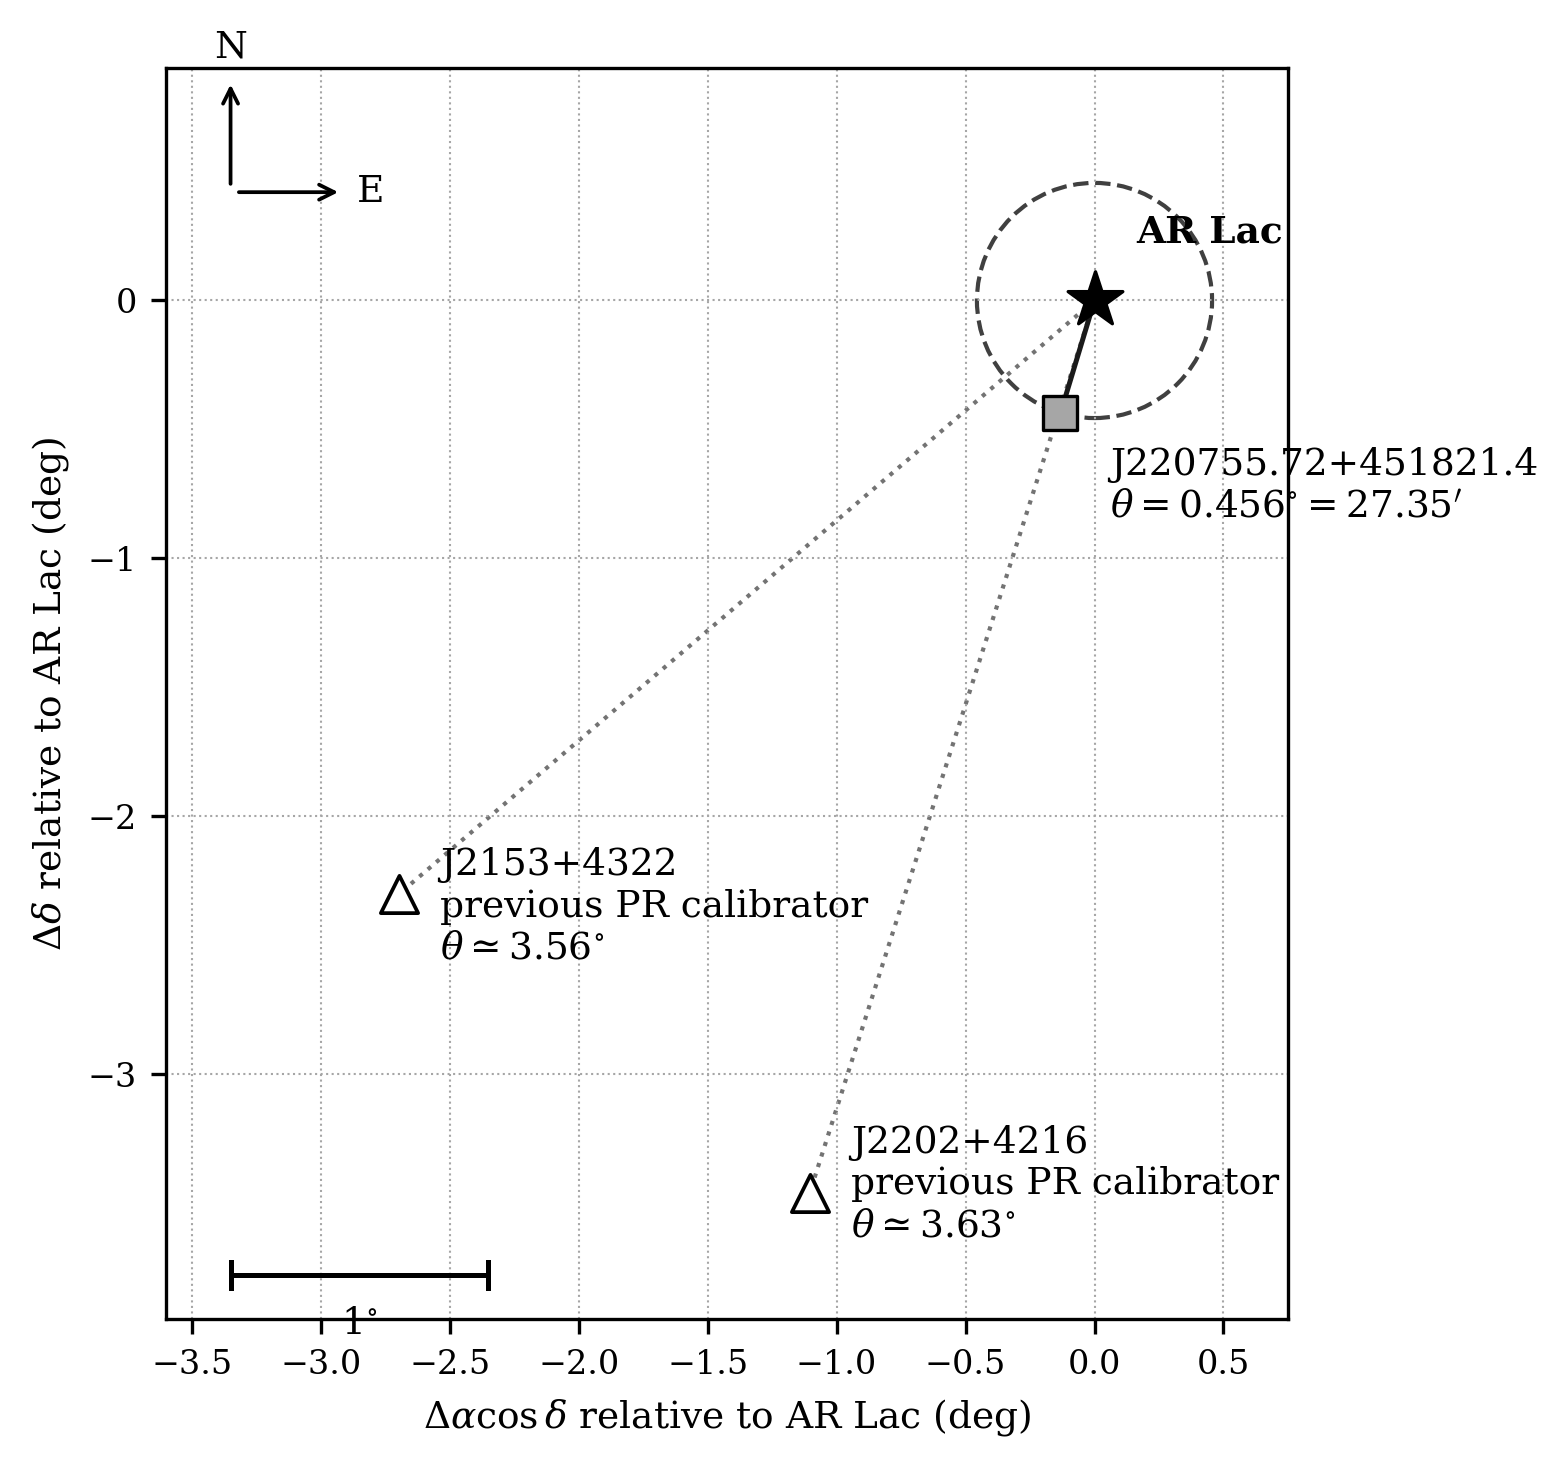
\includegraphics[width=0.60\linewidth]{imgs/arlac_calibrator_geometry.png}
  \caption{AR Lac 与候选近场参考源的相对位置示意图。}
  \label{fig:arlac_calibrator_geometry}
\end{figure}

如表~\ref{tab:radio_flux} 所示。
\begin{table}[htbp]
\centering
\caption{候选参考源的射电流量密度示例。}
\label{tab:radio_flux}
\begin{tabular}{lcc}
\toprule
巡天/目录 & 频率/GHz & 流量密度/mJy \\
\midrule
LoTSS & 0.144 & 25.7 \\
NVSS  & 1.4   & 19.8 \\
VLASS & 3.0   & 31.0 \\
\bottomrule
\end{tabular}
\end{table}

% =========================
% （三）研究基础
% =========================
\YNSectionYanjiuJichu

\YNFixedSubItem{1.研究基础与可行性分析（与本项目相关的研究工作积累和已取得的研究工作成绩，研究风险的应对措施等）；}
\input{sections/03_1_jichu_kexingxing.tex}

\YNFixedSubItem{2.工作条件（包括已具备的实验条件，尚缺少的实验条件和拟解决的途径，包括利用全国重点实验室、省部共建重点实验室和省重点实验室等研究基地的计划与落实情况）；}
\input{sections/03_2_gongzuotiaojian.tex}

\YNFixedSubItem{3.正在承担的与本项目相关的科研项目情况（申请人正在承担的与本项目相关的科研项目情况，包括云南省科技厅的项目和国家其他科技计划项目，要注明项目的资助机构、项目类别、批准号、项目名称、获资助金额、起止年月、与本项目的关系及负责的内容等）；}
\input{sections/03_3_zaichengdan.tex}

\YNFixedSubItem{4.完成国家自然科学基金、省科技厅等项目情况（对申请人负责的前一个已资助期满的科技计划项目（项目名称及批准号）完成情况、后续研究进展及与本申请项目的关系加以详细说明。另附该项目的研究工作总结摘要（限500字）和相关成果详细目录）。}
\input{sections/03_4_yiwancheng.tex}

% =========================
% （四）其他需要说明的情况
% =========================
\YNSectionOther

\YNFixedSubItem{1.申请人在撰写本申请书时使用生成式人工智能的情况，请详细说明申请书中使用的位置和内容。}
\input{sections/04_1_ai.tex}

\YNFixedSubItem{2.其他（\textbf{包括但不限于使用以他人名义申报过的申请书\hbox{}}；如有，请详细说明）。}
\input{sections/04_2_other.tex}

% =========================
% 参考文献：放在“二、正文”结束后，“三、个人简历”之前
% =========================
\YNReferences

% 固定模板后置部分：三、个人简历；四、附件；附件材料表
\YNCVAndAttachments

\end{document}